
\chapter{Ion Sources}\label{ch:ion-sources}

It is important to discuss ions and how they are formed such that we can accelerate them and subsequently implant them into a certain material.
The typical ion source is often a plasma ion source.
Properties of plasma like particle density, temperature, or even the geometry of confinement, play an important role on describing the particle beam we want to create.

\section{Plasma Physics Interlude}\label{sec:plasma-physics-interlude}
\epigraphfontsize{\small\itshape}
\epigraph{ A plasma is a quasi-neutral gas of charged and neutral particles which exhibit collective behaviour. }.

The particle density inside a plasma is made up of three different species: ions, electrons, and neutrals, each with their respective densities $n_i$, $n_e$, $n_n$.
An important parameter of plasma is that of charge quasi-neutrality, so the sum of all the charges should reach 0.
\[ \sum_j Q_j n_j = 0\]
It has often been said that 99\% of the matter in the universe is in the plasma state, and thus it seems we live in the 1\% of the universe in which plasmas do not occur naturally.
The reason for this can be seen from the Saha equation~\ref{eq:saha}, which tells us the amount of ionization to be expected in a gas in thermal equilibrium:

\begin{equation}
	\frac{n_i}{n_n} \approx 2.4\times 10^{15} \frac{T^{3/2}}{n_i} e^{-U_i / k_B T}
	\label{eq:saha}
\end{equation}

where $T$ is the gas temperature in Kelvin, $k_B$ is Boltzmann's constant, and $U_i$ is the ionization energy of the gas (amount of energy required to remove the outermost electron).
For ordinary air at room temperature, the fractional ionization predicted by~\ref{eq:saha} is ridiculously low: $\frac{n_i}{n_n} \approx 10^{-122}$.
One has typically in ion sources less than 10\% of atoms ionized, i.e.,
\[ \frac{n_i}{n_i + n_n} \approx \frac{n_i}{n_n} \leq 0.1 \]

The particle temperature for each of these species is normally given in eV (1 eV $\approx 11,600$ K), and although the specie temperatures may not be the same $(T_i \neq T_e)$, they can still be described by Maxwell distributions.
It is important in ion sources that the $T_i$ is as low as possible, as this will yield a 'better' beam for reasons outlined later.
\subsection{Debye Shielding}\label{subsec:debye-shielding}
A fundamental characteristic of the behaviour of a plasma is its ability to shield out electric potentials that are applied to it.
However, it is not so easy for this energy to be transferred from electron to ion, as within the plasma there is not only particle interaction, but also a phenomenon called shielding.
The interactions of the particles are due to the EM fields they produce because the particles are charged, and thus at microscopic scale, a positive charged ion will be surrounded by negatively charged electrons (shielded), and another positively charged ion further away will not be influenced that much (repulsive force is negligible) by the shielded particle ion.
This concept is quantified by a quantity called the screening distance (also called the Debye length) $\lambda_D$, and is visualized in Figure~\ref{fig:debye}.
\begin{figure}
	\centering
	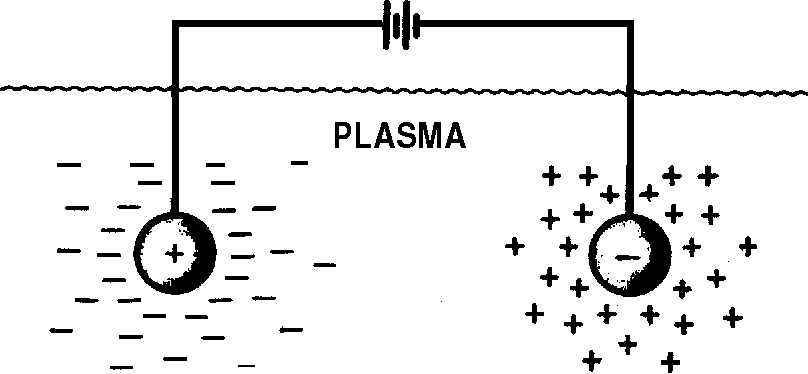
\includegraphics[scale=0.25]{debye}
	\caption{Debye Shielding of a positive charged ion in a plasma due to the collection of negatively charged electrons surrounding it~\cite{chen}.}
	\label{fig:debye}
\end{figure}
Typically the penetration of an external EM field into a plasma is given by the exponential decay $ \approx e^{-x/\lambda_D}$.
This length also describes the decay of the plasma potential $\Phi$ as it reaches a wall/boundary, meaning we must also take into account the material-plasma interface (PWI).
Typically the ions have a lower velocity than the electrons, therefore the electrons leave the plasma at a higher rate than the ions $(v_e \gg v_i)$.
This leads the plasma to be positively charged, and you will have always positively charged plasma and negatively charged walls.
The issue of charge neutrality is also a problem of plasma oscillations.
Although there is shielding, there is still interaction between ions.
One assumes in a plasma, as stated before, a quasi neutrality, i.e., if we split up the plasma into small subsections, those subsections would all be charge neutral, therefore there will be no interaction between the different regions.
The dimension of such a region is given by $\lambda_D$.

Every region described by the debye length can have some local space charges, but over the whole area the local charges cancel out leading to a charge neutrality.
If we have a dimension that is greater than the debye length, we will have charge neutrality ($x \geq \lambda_D$), and for regions smaller, we have both local and temporal fluctuations of charge ($x\leq \lambda_D$).
Within these regions smaller than the debye length, the coulomb force which pulls electrons (being much smaller in mass than the ions) resulting in an oscillatory behaviour of the particles.
Typical values of the debye length are given below:
\begin{center}
\begin{tabular} { |c |c|c|c|}
	\hline
	Plasma & $n_e (m^{-3})$ & $T_e$ & $\lambda_D$  (m) \\
	\hline
	Solar core & $10^{32}$ & $10^7$ &  $10^{-11}$ \\
	\hline
	Tokamak & $10^{20}$ & $10^8$ & $10^{-4}$ \\
	\hline
	Gas discharge & $10^{16}$ & $10^4$ & $10^{-4}$ \\
	\hline
	Interstellar Medium & $10^{4}$ & $10^4$ & $10$ \\
	\hline
\end{tabular}
\end{center}
So we are now in a position to define quasi-neutrality.
If the dimensions $L$ of a system are much larger than $\lambda_D$, then whenever local concentrations of charge arise or external potentials are introduced into the system, these are shielded out in a distance short compared to $L$, leaving the bulk of the plasma free of large electric potentials or fields.
That is, one can take $n_i \approx n_e \approx n$, where $n$ is a common density called the $\textit{plasma density}$, but not so neutral that all the interesting electromagnetic forces vanish.
Thus, the criterion for a plasma is that it be dense enough that $\lambda_D \ll L$.

\subsection{General Criterion for a Plasma}\label{subsec:general-criterion-for-a-plasma}
We have given two of three conditions of an ionized gas in order for it to be considered a plasma.
The final has to do with collisions.
By ionizing particles, we are directly influencing the particle temperature which is then related to the relaxation time(s).
An example of a relaxation time is the $90^{\circ}$ reflection time, which is the time it takes for a particle to be reflected $90^\circ$, and is not produced by a single collision, but rather a high number of small collisions summed up.
This is vastly different from the interaction of particles in gasses or solids.
Another important relaxation time is the energy relaxation time, which is the time for an energy transfer between an electron to an ion.
Plasma heating is done by externally heating electrons, and this energy needs to be transferred to the ions, so of course the time it takes for this equilibrium to be achieved is important when it comes to ion beam preparation.
Due to the different masses and densities of particles in the plasma, one must also distinguish the frequency of the oscillations of electrons and ions.
There are natural modes to these oscillations, so if we consider a single positively charged ion with a nearby electron, the electron will move much faster than the ion and overshoot the ion, and the process repeats with pulling the electron back.
This frequency of the oscillatory behaviour is described as the plasma frequency $\omega_p$, and is split into two, for the electrons $\omega_{pe}$ and for the ions $\omega_{pi}$.
\begin{gather*}
    \omega_{pe}^2 = \frac{e^2 n_e}{\epsilon_0 m_e} \approx GHZ\\
    \omega_{pi}^2 = \frac{(Ze)^2 n_i}{\epsilon_0 m_i} \approx MHz\\
\end{gather*}
Typically $\omega_{pe} > \omega_{pi}$ because of their mass difference.
If we have $\omega$ as the general frequency of the plasma, and $\tau$ is the mean time between collisions (relaxation time), we require that $\omega \tau > 1$ for the gas to behave like a plasma rather than a neutral gas.
The three conditions a plasma must satisfy are therefore:
\begin{myitemize}
	\item 1: $\lambda_D \ll L $
	\item 2: $N_D \gg 1$, where $N_D = n\frac{4}{3} \pi \lambda_D^3$, i.e., the Debye sphere
	\item 3: $\omega \tau > 1$
\end{myitemize}

\section{Ionize the particles}\label{sec:ionize-the-particles}

The question remains, how to we ionize these particles?
We know that we need to apply some amount of energy to kick the electrons away from the particles, but how much energy?
Are certain elements `better' for ionization than others? Why?
The ionization energy for different atoms varies, but follows along the periodic table, as one can see in Figure~\ref{fig:ionization_graph}.

\begin{figure}
	\centering
	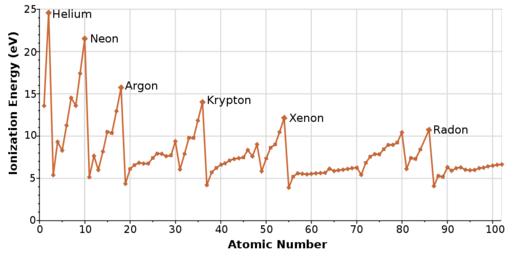
\includegraphics[width=0.8\linewidth, height=5cm]{ionization_energy_plot}
	\caption{Various ionization energies of elements.}
	\label{fig:ionization_graph}
\end{figure}


One idea to ionize atoms is through their impact via electrons.
This is possible if the energy of the electron $E_e$ is greater than or equal than the ionization potential $\Phi_i$, i.e., $E_e \geq e\Phi_i$.
Although it is possible, it is very difficult, as even then we are still working with probabilities.
For max ionization probability, we need an energy 3--4 times greater than the value of the ionization potential, so the maximum probability for ionization will decrease with higher energies.
The energy of electrons is maxwell distributed, which means that the mean energy of electrons in the plasma is given by $\langle E_e \rangle \approx \frac{3}{2} k_b T$.
If we had an ionization potential on the order of 15 eV, then we would need a very high temperature for the electrons, which normally has a range of $T_e \approx 1-10 eV$.
Due to this distribution of temperature of the electrons, it is very unlikely that we should have an electron with this temperature, and additionally this method is not very scalable.
Another idea is to use photon ionization, and this is only possible if the energy of the photon is higher than the ionization energy, $\hbar \nu \geq e\Phi_i$.
However, this is also difficult, for if we had an ionization energy of something as low as 10 eV, we would need to be using UV or x-rays to ionize the particles.
Note: This is different from laser ionized plasmas.
Aside from electron impacts within a plasma, there is also ion impacts.
This turns out to have a very low cross section and therefore not very relevant for ion sources.
It is just relevant if the speed of the ion to collide is equal to the speed of the electron on the shell of the ion, which could be on the order of 100keV. One could also use EM fields to ionize particles.
Imagine a needle with a tip that has very intense EM fields ($1.5\times 10^{10}$ V/m), which leads to an ion extraction, this is used in liquid metal sources like Gallium, or Bismuth, to wet the tip of the needle to extract the ions of these metals from the tip.
The nice aspect of the field ionization is the needle spot accuracy, being about 100 angstrom in size, leading to a great advantage in beam size having the same order of needle tip.
Besides that, one could have a beam current of up to 1 $\frac{A}{cm^2}$ which is quite nice and can be seen in Fig~\ref{fig:fib}.
\begin{figure}

	\centering
	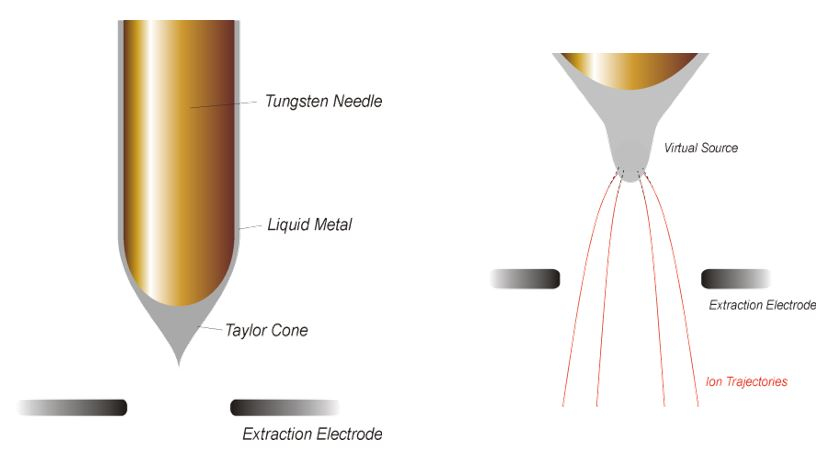
\includegraphics[width=0.8\linewidth, height=5cm]{FIB}
	\caption{During operation, gallium ions flow from a reservoir to the needle apex and a large negative voltage is applied between this needle and an extraction electrode. The balance between the electrostatic forces and the surface tension of gallium wetting the tapered W needle geometry results in the formation of a typical shape of the liquid, named Taylor cone with a half angle of 49.3°. For a typical emission current of $2\mu A$, the cone is distorted and a cusp is formed at the apex of the Taylor cone with a diameter of approximately $5 nm$. At the apex of this cusp the electric field is of the order of $1.5\times 10^{10} V/m$ sufficient to extract the ions by field emission.}
	\label{fig:fib}
\end{figure}

A main component of an ion source is something called an extractor, in which the idea is to have a confined plasma with a small aperture on one edge of it.
Near the aperture, you have a positive voltage that leads to ions to be lead out of the source, followed by a negative voltage to accelerate those extracted.
Normally with an ion beam you would use a single aperture design for a small round beam.
In order to use this beam you need a vacuum for it to travel through, with minimum pressure of $\approx 10^{-6} mbar$.
The energy of the ions extracted is given by the potential voltage of the extractor, $U_{ps}$, i.e.,  $ E_i = eZ (U_{ps} - U_{ch}) \approx eZU_{ps}$.
The reason for the dropout of the chamber voltage, is because it is normally grounded.
Due to the Debye penetration depth, and the tail speed of the electrons, the potential of the plasma is always positive, so $\Phi \approx 10V$ should also be accounted for in our equations, but the extractor voltage is normally on the order of 10 keV, so we can neglect the plasma potential.
The confinement of the plasma in the plasma source is normally done by magnetic confinement via two magnetic mirrors.
The idea is to have the increasing of a magnetic field strength at two ends of a 'bottle' causes a reflection of the ions back towards the confinement.

\subsection{Beam Parameters}\label{subsec:beam-parameters}
Once we have the ion beam generated by the ion extractor, there are a few parameters we are interested in that will determine the effects the beam.
The ion kind, if it is a gas, metal, if it is atomic or molecular in scale ($N_1^+, N_2^+$), what charge state it has $N^+, N^{++}$,  or if it is a mixture, like "Wienfilter",
the current of the ion beam, DC or pulsed ($\approx ms - ns$),
the beam energy (the energy per ion could be anywhere between eV, keV, MeV, but for example at the LHC it is TeV), which can have a magnitude between fA to mA,
the beam current, which is divided into two, the electrical current of the charges $I_e$ traveling in the beam, and the particle current $I_{par}$.
The relation of the two is: $I_e = QI_{par}$ where $Q$ is the charge state of the ion extracted (can be $Z$),
Beam shape/size is also important, as well as the beam divergence (path of beam diverges from the straight line, having an angle $\theta = 2arctan(\frac{D_f - D_i}{2l})$ where $D_i$ is the initial radius of the beam and $D_f$ is the final divergence of the beam and $l$ is the length between those two radii).


\section{Types of Ion Sources}\label{sec:types-of-ion-sources}

A sample list of ion sources is given below:
\begin{myitemize}
	\item RF ion source: one can achieve beam currents on the order of $100 \mu A$, and in principle any gas can be used.
	\item Duoplasmatron
	\item Electron Cyclotron Resonance (ECR)
	\item Single Ion Source (eg., FIB)
\end{myitemize}
All have their own benefits and are used mainly depending on which problem you wish to solve.

\section{Summary of Chapter 2}\label{sec:summary-of-chapter-2}

\begin{myitemize}
	\item Ion sources rely on plasma, and parameters of the plasma like debye shielding $\lambda_D$ play a role on the type of beam created
	\item Generating the plasma is not so simple, but can be done using either electron or photon interactions, or high EM fields (FIB)
	\item One must confine the generated plasma, traditionally done with magnetic mirrors
	\item Finally one must extract the plasma from its confinement, typically done with extractors
	\item All of these steps combine into what we call ion sources
\end{myitemize}
